%% Copernicus Publications Manuscript Preparation Template for LaTeX Submissions
%% ---------------------------------
%% This template should be used for copernicus.cls
%% The class file and some style files are bundled in the Copernicus Latex Package, which can be downloaded from the different journal webpages.
%% For further assistance please contact Copernicus Publications at: production@copernicus.org
%% https://publications.copernicus.org/for_authors/manuscript_preparation.html

%% copernicus_rticles_template (flag for rticles template detection - do not remove!)

%% Please use the following documentclass and journal abbreviations for discussion papers and final revised papers.

%% 2-column papers and discussion papers
\documentclass[soil, manuscript]{copernicus}



%% Journal abbreviations (please use the same for preprints and final revised papers)

% Advances in Geosciences (adgeo)
% Advances in Radio Science (ars)
% Advances in Science and Research (asr)
% Advances in Statistical Climatology, Meteorology and Oceanography (ascmo)
% Aerosol Research (ar)
% Annales Geophysicae (angeo)
% Archives Animal Breeding (aab)
% Atmospheric Chemistry and Physics (acp)
% Atmospheric Measurement Techniques (amt)
% Biogeosciences (bg)
% Climate of the Past (cp)
% DEUQUA Special Publications (deuquasp)
% Earth Surface Dynamics (esurf)
% Earth System Dynamics (esd)
% Earth System Science Data (essd)
% E&G Quaternary Science Journal (egqsj)
% EGUsphere (egusphere) | This is only for EGUsphere preprints submitted without relation to an EGU journal.
% European Journal of Mineralogy (ejm)
% Fossil Record (fr)
% Geochronology (gchron)
% Geographica Helvetica (gh)
% Geoscience Communication (gc)
% Geoscientific Instrumentation, Methods and Data Systems (gi)
% Geoscientific Model Development (gmd)
% History of Geo- and Space Sciences (hgss)
% Hydrology and Earth System Sciences (hess)
% Journal of Bone and Joint Infection (jbji)
% Journal of Micropalaeontology (jm)
% Journal of Sensors and Sensor Systems (jsss)
% Magnetic Resonance (mr)
% Mechanical Sciences (ms)
% Natural Hazards and Earth System Sciences (nhess)
% Nonlinear Processes in Geophysics (npg)
% Ocean Science (os)
% Polarforschung - Journal of the German Society for Polar Research (polf)
% Primate Biology (pb)
% Proceedings of the International Association of Hydrological Sciences (piahs)
% Safety of Nuclear Waste Disposal (sand)
% Scientific Drilling (sd)
% SOIL (soil)
% Solid Earth (se)
% State of the Planet (sp)
% The Cryosphere (tc)
% Weather and Climate Dynamics (wcd)
% Web Ecology (we)
% Wind Energy Science (wes)

% Pandoc citation processing

% The "Technical instructions for LaTex" by Copernicus require _not_ to insert any additional packages.
% % % From pandoc table feature
% \usepackage{longtable,booktabs,array}
% % \usepackage{calc} % for calculating minipage widths
% % Correct order of tables after \paragraph or \subparagraph
% \usepackage{etoolbox}
% \makeatletter
% \patchcmd\longtable{\par}{\if@noskipsec\mbox{}\fi\par}{}{}
% \makeatother
% % Allow footnotes in longtable head/foot
% \IfFileExists{footnotehyper.sty}{\usepackage{footnotehyper}}{\usepackage{footnote}}
% \makesavenoteenv{longtable}
% 
% tightlist command for lists without linebreak
\providecommand{\tightlist}{%
  \setlength{\itemsep}{0pt}\setlength{\parskip}{0pt}}


%
%% \usepackage commands included in the copernicus.cls:
%\usepackage[german, english]{babel}
%\usepackage{tabularx}
%\usepackage{cancel}
%\usepackage{multirow}
%\usepackage{supertabular}
%\usepackage{algorithmic}
%\usepackage{algorithm}
%\usepackage{amsthm}
%\usepackage{float}
%\usepackage{subfig}
%\usepackage{rotating}

\begin{document}


\title{Wall-to-wall mapping of peat depth from Lidar terrain and airborne radiometrics in Norwegian landscapes}


\Author[1][julien.vollering@hvl.no]{Julien}{Vollering}
\Author[2]{Naomi}{Gatis}
\Author[1]{Mette}{Kusk Gillespie}
\Author[1]{Karl-Kristian}{Muggerud}
\Author[1]{Sigurd Daniel}{Nerhus}
\Author[1]{Knut}{Rydgren}
\Author[1]{Mikko}{Sparf}


\affil[1]{Department of Civil Engineering and Environmental Sciences, Western Norway University of Applied Sciences, Norway}
\affil[2]{Department of Geography, University of Exeter, United Kingdom}

\runningtitle{Peat depth from terrain and radiometrics}

\runningauthor{Vollering et al.}


\correspondence{Julien\ Vollering\ (julien.vollering@hvl.no)}



\received{}
\pubdiscuss{} %% only important for two-stage journals
\revised{}
\accepted{}
\published{}

%% These dates will be inserted by Copernicus Publications during the typesetting process.


\firstpage{1}

\maketitle


\begin{abstract}
The abstract goes here.
It can also be on \emph{multiple lines}.
\end{abstract}




\section{Introduction}

Introduction text goes here.
Read Gatis et al. \citeyearpar{gatisMappingUplandPeat2019} and related work \citep{minasnyDigitalMappingPeatlands2019}.

\section{Materials and methods}

\subsection{Sites}

We assessed how well we could predict peat depth at two sites with conspicuously different physical geography: Skrimfjella in eastern Norway and Ørskogfjellet in western Norway (Fig. \ref{fig:sites}c).
These sites were chosen because they were covered by radiometric data from airborne surveys, relatively little built-up area, and road access.

\begin{figure}
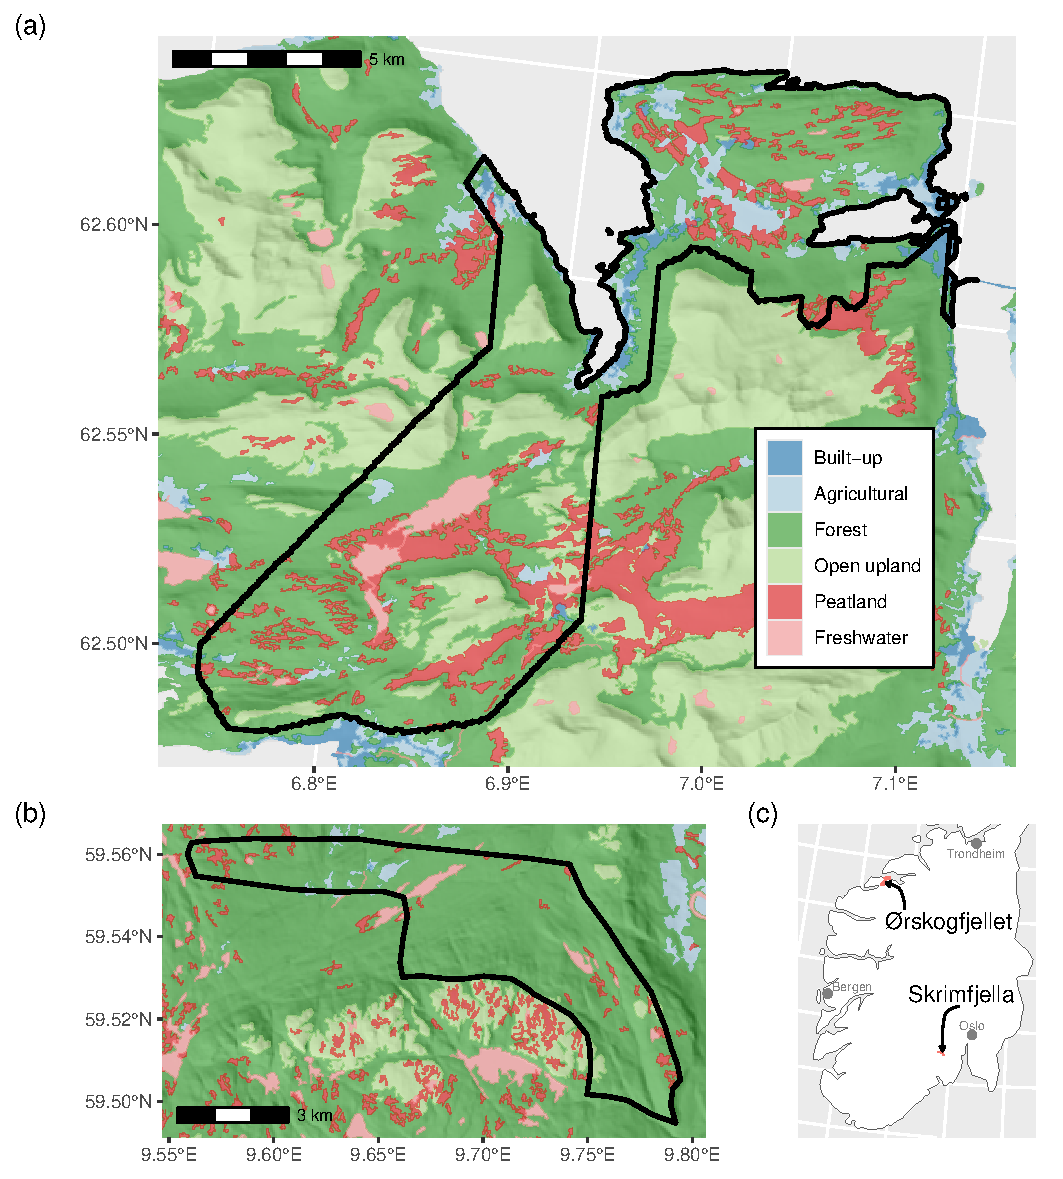
\includegraphics[height=0.9\textheight]{figures/sites-patchwork} \caption{Study areas at Ørskogfjellet (a) and Skrimfjella (b) within southern Norway (c). Land cover shown here is from the AR50 national land resource database and has simplified geometry with respect to the AR5 database used in the study.}\label{fig:sites}
\end{figure}

At Skrimfjella we delineated a study area of \unit{34\,km^{2}} based on radiometric coverage and accessibility (Fig. \ref{fig:sites}b).
The study area has a diverse bedrock, with 32 \% alkali feltspat granite, 26 \% mergelstein, 10 \% granite, and eight other types with \textgreater{} 1 \% coverage (NGU, 1:250 000 dataset).
The landscape within our delineation is classified as \emph{inland hills and mountains} \citep{simensenDiversityDistributionLandscape2021}.
It is almost without human infrastructure, dominated by forest, and borders on a large nature reserve.
The study area has a mean elevation of \unit{438\,m} above sea level (range 223--711, IQR 351--509), and its mean slope at \unit{10\,m} resolution is 10.8° (IQR 4.6--15.1°).
In Norway's AR5 national land capability dataset \citep{ahlstromAR5Klassifikasjonssystem2019}, \unit{1.5\,km^{2}} (4.5 \%) of the study area is classified as mire --- defined as areas with mire vegetation and at least \unit{30\,cm} of peat depth.

At Ørskogfjellet we defined a study area of \unit{124\,km^{2}} which basically followed the footprint of the radiometric survey (Fig. \ref{fig:sites}a).
According to the Geological Survey of Norway, bedrock in the area is 84 \% granitic gneiss, 11 \% granite, and 5 \% aluminium silicate gneiss (NGU, 1:250 000 dataset).
This study area comprises a wide range of major landscape types: \emph{coastal plains}, \emph{coastal fjord}, \emph{inland valleys}, as well as \emph{inland hills and mountains} \citep{simensenDiversityDistributionLandscape2021}.
It is mostly forested, but also contains considerable farmland and open upland, and has several large lakes.
Its mean elevation is \unit{211\,m} above sea level (range 0--807, IQR 73--310), and its mean slope at \unit{10\,m} resolution is 13.0° (IQR 4.7--18.3°).
The AR5 dataset counts \unit{15.3\,km^{2}} (12.4 \%) of the study area as mire.

\subsection{Peat depth measurements}

At both study sites, our measurements of peat depth were made for the purpose of training a Random Forest model of peat depth, and we designed our sampling with this in mind \citep{brusSamplingDigitalSoil2019}.
Broadly, we aimed for a sample that was representative the predictor space of the most important predictors of peat depth \citep{wadouxSamplingDesignOptimization2019, maComparisonConditionedLatin2020}.
A sample that preserves the properties of the multivariate distribution of predictor and outcome variables is most likely to maintain any complex, non-linear relationships that exist in the population while avoiding spurious ones \citep{brusSamplingDigitalSoil2019}.
We chose for our sampling and modelling a spatial resolution of \unit{10\,m}.
We considered this a reasonable compromise between digital terrain model (DTM) resolution (\unit{1\,m}) and small mires on the one hand, and airborne radiometric resolution (\unit{50\,m}) on the other.

\subsubsection{Skrimfjella}

We measured peat depth in selected locations (\unit{10\,m} raster cells) at Skrimfjella.
The locations were chosen only from areas delineated as mire in the AR5 national land capability dataset.
Within this mire area, we stratified our sample across values of elevation, slope, and potassium ground concentration \citep[from processed airborne gamma ray spectrometry,][]{baranwalHelicopterborneMagneticElectromagnetic2013}.
Specifically, we used the \emph{eSample} function in the \emph{iSDM} R package (v.1.0) to chose an environmentally systematic sample.
This function defines the environmental space as a two-dimensional convex hull around the ordinated data, then creates a regular grid across that space, and lastly finds for each grid cell the datum that is nearest \citep{hattabUnifiedFrameworkModel2017}.
Elevation was extracted from the \unit{10\,m} national DTM, slope calculated in degrees, and potassium ground concentration downscaled with bilinear resampling.
We set a target sample size of 100, excluded the top and bottom percentile from the convex hull, and with these parameters \emph{eSample} returned 105 raster cells.

In addition to the peat depth locations, we had another arm of our sampling design for measuring peatland occurrence, as binary variable.
We wanted to measure peatland occurrence outside of mapped mire areas because the AR5 dataset is known to underestimate peatland coverage \citep[especially in forests,][]{brynLandCoverNorway2018}, and because airborne radiometrics may help identify unmapped peatland \citep{gatisMappingUplandPeat2019, olearyDigitalSoilMapping2022}.
The occurrence locations were sampled from the part of the study area that (1) was mapped as something other than mire in the AR5 database and (2) had a slope \textless{} 20°.
We performed environmentally systematic sampling of this population with the same procedure as for the depth locations, and \emph{eSample} returned 106 raster cells.

Field work at Skrimfjella was conducted in August 2020.
We navigated to the centers of the raster cells in the depth and occurrence samples by handheld GPS, checking that positional error was below \unit{3\,m}.
For each depth sample location, we measured peat depth three times (at the vertices of a triangle with \unit{2\,m} sides) to get a more representative value for the \unit{10\,m} raster cell, and to dampen the effect of outlying measurements \citep{parryEvaluatingApproachesEstimating2014}.
We used a metal probe pushed downward until resistance indicated the base of the peat column.
Probe locations were adjusted up to \unit{20\,cm} if the base of the peat column seemed to be blocked by an obvious artifact.
For each occurrence sample location, we recorded the presence or absence of peatland --- primarily by digging and examining the top \unit{20\,cm} of soil (where this was possible).
We judged whether the soil was a peat soil based on its density, texture, and color.
Occasionally, when the soil itself was difficult to judge, we made our determination also based on the presence or absence of mire vegetation.
Although peat soil is strictly defined by organic content (which we did not analyse), we believe our protocol produced reasonable determinations of presence or absence that would generally satisfy most of the varying definitions of peatland \citep{minasnyMappingMonitoringPeatland2023}.

Besides the depth and occurrence measurements described above, we also measured peat depth in three subjectively-chosen, individual mires, using ground-penetrating radar (GPR).
We used the Malå ProEx GPR system (Guideline Geo AB, Sweden) with its \unit{500\,MHz} shielded antenna mounted in a plastic sledge, and its control unit connected to a GNSS receiver.
At each of the three mires we recorded GPR traces along walking transects that covered the extent of the mire, mostly in traversing, zigzag patterns with between \unit{5\,m} and \unit{20\,m} spacing at their vertices.
Along the GPR transects we also probed peat depth at marked trace locations, to be able to calibrate the GPR wave speed velocity.
We processed the GPR data with Reflex2DQuick software (v.3.0, Sandmeier Scientific Software, Germany), applying a time-zero correction, a dewow filter, and a gain filter based on observed energy decay.
Then we picked strong reflectors in the radargrams that we interpreted as the base of the peat column.
We used picks at marked trace locations to calibrate wave speed velocity; we pooled calibration points across the three mires and fitted a linear regression of depth on one-way travel time with the intercept fixed at zero.
In total we had 46 calibration points along \unit{3.5\,km} of GPR transects.
Finally, we used the calculated wave velocity (\unit{0.0387\,m\,ns^{-1}}, \(R^2 = 0.874\)) to convert the travel times of all picks to calibrated peat depths.

\subsubsection{Ørskogfjellet}

At Ørskogfjellet we also measured peat depth in a sample of \unit{10\,m} raster cells, selected from the part of the study area classified in the AR5 dataset as mire.
Before selecting locations, we determined a minimal sample size that would adequately capture the terrain and radiometric properties of the entire mire area.
Specifically, we aimed to identify the size at which adding locations produced diminishing decreases in divergence between sample and population distributions --- i.e.~the elbow point in a curve of similarity between sample and population \citep{maloneMethodsImproveUtility2019}.
This approach has been found to identify sample sizes that correspond with diminishing returns in predictive model performance on external evaluation data \citep{sauretteDivergenceMetricsDetermining2023}.
We defined a sequence of sample sizes (50--500) and for ten replicate samples at each size \citep[drawn by conditioned latin hypercube sampling,][]{minasnyConditionedLatinHypercube2006, roudierClhsPackageConditioned2011}, we calculated the mean Kullback-Leibler divergence between sample and population distributions \citep{maloneMethodsImproveUtility2019, sauretteDivergenceMetricsDetermining2023}.
The variables in the divergence calculation were terrain slope and four radiometrics: potassium, thorium, uranium, and total count.
Next, we fitted a asymptotic regression of mean divergence on sample size, and identified the sample size at which the curve reached 95 \% of the fitted asymptote.
Through this procedure we found that we could adequately capture the population distribution with a sample of 160 locations.

To choose 160 locations, we performed feature space coverage sampling.
This approach has been found to produce higher accuracy in Random Forest models than conditioned latin hypercube sampling \citep{wadouxSamplingDesignOptimization2019, maComparisonConditionedLatin2020}.
Feature space coverage sampling aims to disperse samples as uniformly as possible in multidimensional predictor space, and is implemented by choosing locations that are closest to cluster centers in a k-means clustering of the standardized predictor space \citep{brusSamplingDigitalSoil2019}.
Feature space coverage sampling works best when all dimensions are important predictors of the outcome \citep{wadouxSamplingDesignOptimization2019}, and we used the same five predictors that we used to choose sample size: terrain slope and four radiometrics.
The radiometric variables were downscaled to \unit{10\,m} resolution with cubic B-spline resampling in QGIS \citep[v.3,][]{QGISsoftware}.
We adjusted the feature space coverage sampling to ensure that locations were accessible within time constraints, and assessed how this changed our sample from an ideal feature space coverage sample.
Adjusting for accessibility is justified because the smaller sample size that would result if accessibility were ignored can degrade model accuracy as much or more as deviations from ideal sampling designs \citep{wadouxSamplingDesignOptimization2019, maComparisonConditionedLatin2020}.
To adjust, we first restricted the sampling population to mire areas that were within an arbitrary cost distance of publicly-accessible roads.
Cost distance was calculated using GRASS's \emph{r.walk} function, with friction costs defined by AR5 land classes \citep{GRASSv8-2}.
After creating a feature space coverage sample with this restriction, we also inspected a map of the sample and substituted 16 inaccessible locations with accessible locations from the same or a nearby cluster.
Our two accessibility adjustments increased the distance in standardized predictor space between sample locations and cluster centers by 78 \% (with respect to the ideal sample), but distance in our sample was still only 46 \% of the mean distance to cluster centers --- i.e., accessibility did not force locations far from cluster centers relative to the size of the clusters.

Field work at Ørskogfjellet was conducted in August 2023.
We navigated to the centers of the raster cells in the sample using real time kinematic differential GNSS (Topcon Positioning Systems, USA), to ensure sub-meter positional accuracy.
At each location we measured peat depth three times by manual probing, with probe locations spaced approximately \unit{2.5\,m} apart.
In areas with dense sampling locations, we also measured peat depth with GPR along snaking transects passing through the centers of the sampling cells (seven transects, \unit{6.2\,km} total length).
We used the same GPR system as at Skrimfjella, but with a \unit{100\,MHz} Malå rough terrain antenna (Guideline Geo AB, Sweden) at some transects.
To navigate the GPR transects, we placed flags at the cell centers of the sample locations, and used a handheld GNSS receiver to guide the GPR operator.
At sampling locations crossed by a GPR transect, we arranged the manual probe positions along the transect (for better calibration of the GPR wave speed velocity), while other locations were probed in a triangular pattern around the cell center like at Skrimfjella.

We processed the GPR data with Reflexw software (v.8.5, Sandmeier Scientific Software, Germany), applying a dewow filter, time-zero correction, bandpass filter, gain filter, and a dynamic correction that accounts for the non-vertical wave path between offset transmitter and receiver antennae.
The last correction is important for the rough terrain antenna, which has an antenna separation (\unit{2.2\,m}) --- comparable to typical peat depths.
As with the data from Skrimfjella, we picked the base of the peat column from strong reflectors in the radargram, and calibrated wave velocity with manual probe measurements in a linear regression.
The points in the regression were created by joining to each probe measurement the travel time of the nearest pick, but only if these were within \unit{2\,m} of each other.
In total we had 78 calibration points along \unit{7.8\,km} of interpretable GPR traces (transect length exceeded because of extra GPR data).
Finally, we used the calculated wave velocity (\unit{0.0427\,m\,ns^{-1}}, \(R^2 = 0.946\)) to convert the travel times of all picks to calibrated peat depths.

We also used two sets of existing depth measurements from Ørskogfjellet.
The first set was provided by the Norwegian Public Roads Administration, who commissioned GPR surveys of particular peatland areas in 2020 and 2021.
The surveys were conducted with a dual channel system (\unit{70\,MHz} and \unit{300\,MHz}; ImpulseRadar AB, Sweden), connected to GNSS with CPOS correction.
We used interpreted and calibrated traces from these surveys, and discarded some data where multiple depths were interpreted for the same locations.
This summed to \unit{7.4\,km} of interpreted traces.
The second set of existing depth data we extracted from a paper map made by the Norwegian Soil and Mire Company in 1984.
This map presents 44 borehole depths (in decimeters) across a \unit{9\,ha} peatland area.
We georeferenced the map and digitized the borehole locations and depths.

\subsection{Peat depth predictors}

We created the same suite of 25 quantitative peat depth predictors for both sites (Table \ref{tab:preds}).
All quantitative predictors were derived either from an airborne radiometric survey or from a DTM.
From the radiometric surveys we simply used the four variables produced by the surveyors (Geological Survey of Norway): ground concentration of Potassium, Thorium, Uranium, as well as total count.
From the DTMs we calculated several land surface parameters, ranging from simple terrain indices to more complex geomorphometric and hydrological variables \citep{maxwellLandsurfaceParametersSpatial2022}.

\begin{table}

\caption{\label{tab:preds}Quantitative predictors of peat depth.}
\centering
\begin{tabular}[t]{l|l}
\hline
name & description\\
\hline
radK & Potassium ground concentration\\
\hline
radTh & Thorium ground concentration\\
\hline
radU & Uranium ground concentration\\
\hline
radTC & Total count of gamma radiation\\
\hline
elevation & Mean elevation\\
\hline
slope1m & Mean of 1 m slope\\
\hline
TPI1m & Mean of 1 m topographic position index\\
\hline
TRI1m & Mean of 1 m terrain ruggedness index\\
\hline
roughness1m & Mean of 1 m roughness\\
\hline
slope10m & 10 m slope\\
\hline
TPI10m & 10 m topographic position index\\
\hline
TRI10m & 10 m terrain ruggedness index\\
\hline
roughness10m & 10 m roughness\\
\hline
MRVBF & Multi-resolution valley bottom flatness\\
\hline
TWI5m & Mean of 5 m topographic wetness index\\
\hline
TWI10m & 10 m topographic wetness index\\
\hline
TWI20m & Bilinear interpolation of 20 m topographic wetness index\\
\hline
TWI50m & Bilinear interpolation of 50 m topographic wetness index\\
\hline
DTW2500 & Depth-to-water index, flow initiation area of 2500 m\textasciicircum{}2\\
\hline
DTW5000 & Depth-to-water index, flow initiation area of 5000 m\textasciicircum{}2\\
\hline
DTW10000 & Depth-to-water index, flow initiation area of 10000 m\textasciicircum{}2\\
\hline
DTW20000 & Depth-to-water index, flow initiation area of 20000 m\textasciicircum{}2\\
\hline
DTW40000 & Depth-to-water index, flow initiation area of 40000 m\textasciicircum{}2\\
\hline
DTW80000 & Depth-to-water index, flow initiation area of 80000 m\textasciicircum{}2\\
\hline
DTW160000 & Depth-to-water index, flow initiation area of 160000 m\textasciicircum{}2\\
\hline
\end{tabular}
\end{table}

The radiometric survey covering Skrimfjella was conducted in 2008--2011.
The survey was flown at an average altitude of \unit{75\,m} and average speed of \unit{108\,km\,h^{-1}}, with flight lines spaced \unit{200\,m} apart.
Spectrometer count rates were calibrated annually to known concentrations of Potassium, Thorium, and Uranium in mobile pads.
The Geological Survey of Norway processed data from the spectrometer following standard procedures outlined by the International Atomic Energy Association, and the processing included: correction for aircraft and cosmic background radiation, correction for radon in the air, window stripping of the gamma ray spectrum, correction for flying height, conversion of count rates to ground concentrations, and finally gridding to \unit{50\,m} resolution with micro-leveling.
Further details about the survey and data processing are provided in Baranwal et al. \citeyearpar{baranwalHelicopterborneMagneticElectromagnetic2013}.
We downscaled the processed data to \unit{10\,m} resolution by cubic spline resampling, using the \emph{terra} package in R.

A very similar radiometric survey covering Ørskogfjellet was conducted in December 2014 and January 2015.
This survey was flown at an average altitude of \unit{80\,m} and average speed of \unit{88\,km\,h^{-1}}, with flight lines also spaced \unit{200\,m} apart.
Spectrometer count rates were calibrated in 2013 to known concentrations of Potassium, Thorium, and Uranium in mobile pads.
The spectrometer data were processed following the same procedure as for the survey at Skrimfjella, except that a convolution filter was added to smooth the gridded data.
Further details about the survey and data processing are provided in Ofstad \citeyearpar{ofstadHelicopterborneMagneticRadiometric2015}.
The \unit{10\,m} resolution predictors from this survey were identical to the layers used in the sampling design (resampled from \unit{50\,m} resolution with cubic B-splines).

For terrain-derived variables, we obtained \unit{1\,m} resolution DTMs from the Norwegian Mapping Authority.
The DTM for Skrimfjella was produced from airborne laser scanning surveys in 2015 and 2022, with laser point density of \unit{5\,pts\,m^{-2}}.
For Ørskogfjellet, the DTM was produced from a 2015 survey with \unit{2\,pts\,m^{-2}}.
Where necessary, DTMs were resampled to the coordinate reference system of the radiometric data.

We used the \emph{terra} R package to calculate from the DTMs: slope, topographic position index (difference from mean of eight neighbors), terrain ruggedness index (mean of absolute differences from eight neighbors), and roughness (range in the nine-cell neighborhood).
These variables were derived at two scales to produce different predictors; we either calculated from \unit{1\,m} DTM resolution and then aggregated, or aggregated to \unit{10\,m} DTM resolution and then calculated the indices.
This kind of multiscale feature engineering of land surface parameters has been found to greatly improve machine learning predictions of soil properties \citep{millerImpactMultiscalePredictor2015, newmanAssessingSpatiallyHeterogeneous2023}.
We chose \unit{1\,m} and \unit{10\,m} resolutions because we know that peat depth tends to vary at fine scales in Norway \citep{maxwellLandsurfaceParametersSpatial2022}.
We also calculated the the Multi-Resolution Valley Bottom Flatness index, which indicates the degree of valley bottom flatness at a given location via a multiscale algorithm \citep{gallantMultiresolutionIndexValley2003}.
We calculated this index in SAGA GIS \citep[v.9.3.2,][]{conradSystemAutomatedGeoscientific2015} with default parameters.

Next, we calculated the Topographic Wetness Index \citep{quinnPredictionHillslopeFlow1991}.
This index is notoriously scale-dependent and often matches real hydrological conditions best when calculated from moderate-to-coarse resolution DTMs \citep{agrenEvaluatingDigitalTerrain2014, riihimakiTopographicWetnessIndex2021}, so we calculated it from \unit{5\,m}, \unit{10\,m}, \unit{20\,m}, and \unit{50\,m} DTM resolution.
The calculations were performed with Whitebox software \citep{lindsayWhiteboxGATCase2016}, accessed through the \emph{whitebox} R package \citep[v2.4,][]{wuWhiteboxWhiteboxToolsFrontend2022}.
We filled depressions in the DTM with the algorithm in Wang \& Liu \citeyearpar{wangEfficientMethodIdentifying2006}, and used the deterministic infinity flow accumulation algorithm \citep{tarbotonNewMethodDetermination1997}.

We also explored one categorical predictor --- peat depth class --- derived from historical map data.

\subsection{Predictive models of peat depth}

\section{Results}

Include a 12cm width figure of Nikolaus Copernicus from \href{https://en.wikipedia.org/wiki/File:Nikolaus_Kopernikus.jpg}{Wikipedia} with caption using R Markdown (Fig. \ref{fig:portrait}).

\begin{figure}
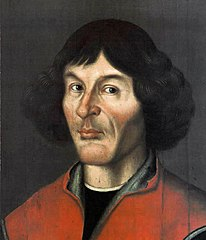
\includegraphics[width=8.3cm]{Nikolaus_Kopernikus} \caption{one column figure}\label{fig:portrait}
\end{figure}

\subsection{Tables}

You can add \LaTeX table in an R Markdown document to meet the template requirements (Table \ref{tab:latextable}).

\begin{table}[t]
\caption{TEXT}
\begin{tabular}{l c r}
\tophline

a & b & c \\
\middlehline
1 & 2 & 3 \\

\bottomhline
\end{tabular}
\belowtable{Table Footnotes}
\label{tab:latextable}
\end{table}

Or you can use markdown to create the table with booktabs = FALSE (\url{https://github.com/rstudio/rticles/issues/558\#issuecomment-1907981541}).

See Table \ref{tab:test}.

\begin{table}

\caption{\label{tab:test}My caption}
\centering
\begin{tabular}[t]{l|r|r|r}
\hline
  & mpg & cyl & disp\\
\hline
Mazda RX4 & 21.0 & 6 & 160\\
\hline
Mazda RX4 Wag & 21.0 & 6 & 160\\
\hline
Datsun 710 & 22.8 & 4 & 108\\
\hline
\end{tabular}
\end{table}

\section{Discussion}

Lorem ipsum dolor sit amet, consectetur adipiscing elit.
Sed do eiusmod tempor incididunt ut labore et dolore magna aliqua.
Ut enim ad minim veniam, quis nostrud exercitation ullamco laboris nisi ut aliquip ex ea commodo consequat.
Duis aute irure dolor in reprehenderit in voluptate velit esse cillum dolore eu fugiat nulla pariatur.
Excepteur sint occaecat cupidatat non proident,
sunt in culpa qui officia deserunt mollit anim id est laborum.

\section{Conclusions}

Nulla facilisi.
Maecenas vel nunc nec purus tincidunt congue.
Proin auctor, lectus eu pharetra malesuada,
nisi nunc bibendum nunc,
eget tincidunt nunc nisi id nunc.
Sed euismod, nunc sit amet aliquam tincidunt,
nunc nunc tincidunt nunc,
nec tincidunt nunc nunc nec nunc.
Donec auctor, nunc sit amet aliquam tincidunt,
nunc nunc tincidunt nunc,
nec tincidunt nunc nunc nec nunc.



\codedataavailability{\emph{Code and data availability.} Use this to add a statement when having data sets and software code available} %% use this section when having data sets and software code available



%%%%%%%%%%%%%%%%%%%%%%%%%%%%%%%%%%%%%%%%%%
%% optional

%%%%%%%%%%%%%%%%%%%%%%%%%%%%%%%%%%%%%%%%%%
\appendix
\section{For submission}

``Appendices: all material required to understand the essential aspects of the paper
such as experimental methods, data, and interpretation
should preferably be included in the main text.
Additional figures, tables, as well as technical and theoretical developments
which are not critical to support the conclusion of the paper,
but which provide extra detail and/or support useful for experts in the field
and whose inclusion in the main text would disrupt the flow of descriptions or demonstrations
may be presented as appendices.
These should be labelled with capital letters: Appendix A, Appendix B etc.
Equations, figures and tables should be numbered as (A1), Fig. B5 or Table C6, respectively.
Please keep in mind that appendices are part of the manuscript
whereas supplements (see below) are published along with the manuscript.''

\section{Figures and tables in appendices}

Please also sort the appendix figures and appendix tables into the respective appendix sections.
They will be correctly named automatically.

\section{Copernicus from Rmarkdown}

\textbf{Please note:} Per \href{https://publications.copernicus.org/for_authors/manuscript_preparation.html}{their guidelines},
Copernicus does not support additional \LaTeX{} packages
or new \LaTeX{} commands than those defined in their \texttt{.cls} file.
This means that you cannot add any extra dependencies
and a warning will be thrown if so.
\textbf{Important}: Always double-check with the official manuscript preparation guidelines
at \url{https://publications.copernicus.org/for_authors/manuscript_preparation.html},
especially the sections ``Technical instructions for LaTeX'' and ``Manuscript composition''.
Please contact Daniel Nüst, \texttt{daniel.nuest@uni-muenster.de}, with any problems.
\noappendix

%%%%%%%%%%%%%%%%%%%%%%%%%%%%%%%%%%%%%%%%%%
\authorcontribution{\emph{Author contributions.}
JV: Conceptualization, Investigation, Data curation, Formal analysis, Writing -- original draft.
NG: Conceptualization, Methodology, Writing - review \& editing.
MKG: Investigation, Writing - review \& editing.
KKM: Investigation, Data curation, Writing - review \& editing.
SDN: Investigation, Writing - review \& editing.
KR: Conceptualization, Investigation, Writing - review \& editing.
MS: Investigation, Data curation, Writing - review \& editing.} %% optional section

%%%%%%%%%%%%%%%%%%%%%%%%%%%%%%%%%%%%%%%%%%
\competinginterests{\emph{Competing interests.} The authors declare that they have no conflict of interest.} %% this section is mandatory even if you declare that no competing interests are present

%%%%%%%%%%%%%%%%%%%%%%%%%%%%%%%%%%%%%%%%%%
\disclaimer{\emph{Disclaimer.} The authors declare that the results, discussions, and interpretations presented in this study are solely their own. The views expressed herein do not necessarily reflect those of their respective institutions or funding agencies.} %% optional section

%%%%%%%%%%%%%%%%%%%%%%%%%%%%%%%%%%%%%%%%%%
\begin{acknowledgements}
\emph{Acknowledgements.} We thank the Norwegian Public Roads Administration for sharing data from ground-penetrating radar surveys. We also thank Vikas Baranwal from the Geological Survey of Norway for helping us access the radiometric data from Skrim. This work contains data under the following licenses: (1) Creative Commons Attribution 4.0 International, © Kartverket, (2) \emph{Norge digitalt} license, Norwegian Institute of Bioeconomy Research (NIBIO), © Geovekst, and (3) the Norwegian License for Public Data (NLOD), made available by the Geological Survey of Norway (NGU).
\end{acknowledgements}

%% REFERENCES
%% DN: pre-configured to BibTeX for rticles

%% The reference list is compiled as follows:
%%
%% \begin{thebibliography}{}
%%
%% \bibitem[AUTHOR(YEAR)]{LABEL1}
%% REFERENCE 1
%%
%% \bibitem[AUTHOR(YEAR)]{LABEL2}
%% REFERENCE 2
%%
%% \end{thebibliography}

%% Since the Copernicus LaTeX package includes the BibTeX style file copernicus.bst,
%% authors experienced with BibTeX only have to include the following two lines:
%%
\bibliographystyle{copernicus}
\bibliography{ms.bib}
%%
%% URLs and DOIs can be entered in your BibTeX file as:
%%
%% URL = {http://www.xyz.org/~jones/idx_g.htm}
%% DOI = {10.5194/xyz}


%% LITERATURE CITATIONS
%%
%% command                        & example result
%% \citet{jones90}|               & Jones et al. (1990)
%% \citep{jones90}|               & (Jones et al., 1990)
%% \citep{jones90,jones93}|       & (Jones et al., 1990, 1993)
%% \citep[p.~32]{jones90}|        & (Jones et al., 1990, p.~32)
%% \citep[e.g.,][]{jones90}|      & (e.g., Jones et al., 1990)
%% \citep[e.g.,][p.~32]{jones90}| & (e.g., Jones et al., 1990, p.~32)
%% \citeauthor{jones90}|          & Jones et al.
%% \citeyear{jones90}|            & 1990


\end{document}
